\documentclass[10pt,a4paper]{article}
\usepackage[utf8]{inputenc}
\usepackage{amsmath}
\usepackage{amsfonts}
\usepackage{amssymb}
\usepackage{graphicx}
\usepackage{amsthm}
\begin{document}
% Actually, we're looking at J_t^j->inf(x) instead of Q^j(x). Does this make a big difference?
\section{RLMPC proof}
Note: Idea: Only use stacked iterations which are "interrupted" in the middle to get the new initial state. Prove that this yields decreasing stacked cost. Might need extra assumptions. Problem: Comparing stacked cost doesn't make sense. We are always only interested in the first lap, so if the improvement shows only in the second lap it won't help us at all. So instead, we will need to compare always only the first of these two stacked iterations and show that their cost are decreasing. Next problem: Consecutive laps probably don't necessarily need to be decreasing. \\
Main idea: Stack laps together (e.g. laps 1+2, 2+3, ...) and construct stacked iteration costs and Q functions. Then use the initial state (e.g. $x_0^2$ of laps 2+3) of one stack, which is the "middle state" of the previous stack (of laps 1+2), to prove that the stacked iteration cost of two consecutive stacks is non-decreasing.\\\\
Define the single iteration cost as usual:
\begin{align}
J^j&=J^j_{0\rightarrow\infty}=\sum_{t=0}^\infty h(x_t^j,u_t^j)\\
h(x,u)&=0\ \forall\ x>P
\end{align}
Additionally, define cost of two consecutive iterations:
\begin{equation}
J^{jk}=J^j+J^{k}=\sum_{t=0}^\infty h(x_t^j,u_t^j)+\sum_{t=0}^\infty h(x_t^{k},u_t^{k})
\end{equation}
with $k = j+1$.\\
Also define the Q function as usual and additionally the Q function of two consecutive iterations:
% Add standard definition of Q for 2 consecutive laps!! Maybe need to show that it is the same as the equation below?
\begin{align}
Q^{jk}(x)&=\begin{cases}
Q^j(x)+J^k, & \text{if $0\leq x<P$}.\\
Q^k(x-P), & \text{if $P\leq x<2P$}.
\end{cases}
\end{align}
with $P=$ periodicity and two consecutive iterations $j$ and $k$. See fig. \ref{fig:proof} for the illustration of these stacked functions.\\
This stacked Q function just adds the Q functions of two consecutive iterations (with $Q=0$ at $x=2P$).\\
Then we can write the optimal LMPC cost for two consecutive laps 2 and 3 as follows (use 3rd plot in figure, iterations 2 and 3):
\begin{align}
J_{0\rightarrow N}^{*,23}(x_0^2)&=\min_u\left[\sum_{t=0}^{N-1}h(x,u)+Q^{01}(x_N)\right]\\
J_{0\rightarrow N}^{*,23}(x_0^2)&=\min_u\left[\sum_{t=0}^{N-1}h(x,u)+Q^0(x_N)\right]+J^1\label{eq:one}
\end{align}
with $x_N\in [0,P]$.\\
We assume that following equation is still valid:
\begin{equation}
J_{0\rightarrow N}^{*,23}(x_0^2)\geq J^{23}.\label{eq:three}
\end{equation}
We can also express the iteration cost of laps 1 and 2 as
\begin{align}
J^{12}&=J^1+J^2\\
J^{12}&=J^1+\sum_{t=0}^{N-1}h(x-P,u)+Q^0(x_N-P) \label{eq:two}
\end{align}
with $x_N>P$ (see 2nd plot in figure, iterations 1 and 2). \emph{Note:} This comes from the fact that, in iteration 12, we use $Q^{-1,0}$ which is not illustrated in the figure.\\
Comparing eq. \ref{eq:one}, \ref{eq:three}, and \ref{eq:two} leads us to
\begin{equation}
J^{12}\geq J_{0\rightarrow N}^{*,23}(x_0^2) \geq J^{23}\qed
\end{equation}

\begin{figure}[ht]
	\centering
  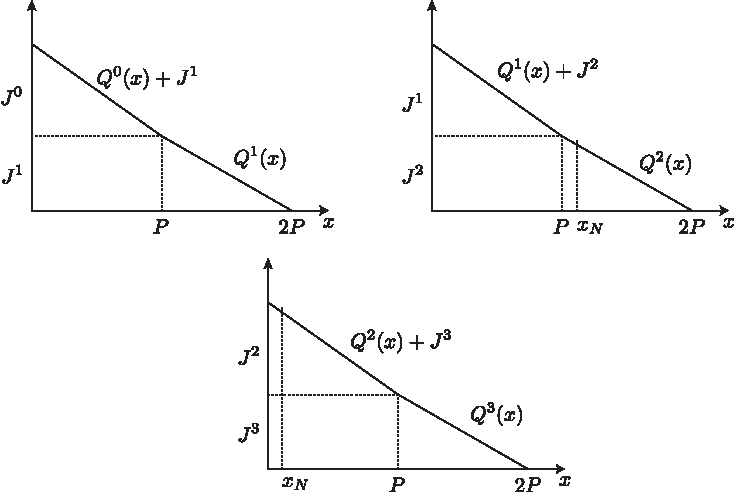
\includegraphics{graph.pdf}
	\caption{Illustration}
	\label{fig:proof}
\end{figure}

\end{document}